\chapter{Codes et Algèbre de Boole}
\section{Code}
Pour pouvoir, en binaire, représenter les chiffres de 0 à 9, il nous faut au minimum 4 bits ($\log_2 10$). Donc, nous perdons 6 codes du à l'arrondissement à 4 bits (1010, 1011, 1100, 1101, 1101 et 1111). En octal et hexadécimal, c'est plus pratique car il n'y a pas de perte du à l'arrondissement ($\log_2 8=3$ et $\log_2 16=4$).Il y a donc, d'autres façons de coder en fonction de l'utilisation qu'on en fait. On en distingue 3 classes: 
\begin{enumerate}
	\item 	Codes pondérés (\textit{weighted codes})
	\begin{itemize}
		\item 8421 \textit{Binary coded Decimal} (BCD) où chaque chiffre est codé séparément
		\item Codes auto-complémentaires
		\begin{itemize}
			\item 2421 Code
			\item Code excédent 3 (Excess 3)
		\end{itemize}
	\end{itemize}
	\item Codes non-pondérés
	\begin{itemize}
		\item Code Gray (code cyclique)
		\item \textit{American Standard Code for Information Interchage} (code ASCII)
	\end{itemize}
	\item Code détecteurs d'erreur
\end{enumerate}
\subsection{Codes pondérés}
Voici une table pour bien comprendre comment fonctionnent les codes auto-complémentaires (le $-$ de $-3$ correspond au chiffre négatif)
\begin{table}[H]
	\centering
	\begin{tabular}{c|c|c|c}
		Décimal & 8421 (BCD) & 2421 & 642-3 \\
		\hline
		0 & 0000 & 0000 & 0000\\
		\hline
		1 & 0001 & 0001 & 0101\\
		\hline
		2 & 0010 & 0010 & 0010\\
		\hline
		3 & 0011 & 0011 & 1001\\
		\hline
		4 & 0100 & 0100 & 0100\\
		\hline
		5 & 0101 & 1011 & 1011\\
		\hline
		6 & 0110 & 1100 & 0110\\
		\hline
		7 & 0111 & 1101 & 1101\\
		\hline
		8 & 1000 & 1110 & 1010\\
		\hline
		9 & 1001 & 1111 & 1111		
	\end{tabular}
	\caption{Code auto-complémentaire}
\end{table}
\subsubsection{Addition en BCD}
L'addition en BCD est simple, on additionne par 4 bits (chaque chiffre composant la base 10). Si le chiffre est $\geq 10$, on ajoute $+6\,(0110)_2$ car cela correspond à un report de 10 en binaire. En effet, regroupé par 4 correspond à de l'hexadécimal, du coup, pour passer de 10 à 0, il faut ajouter 6 ($A\overset{+1}{\rightarrow}B\overset{+1}{\rightarrow}\dots\overset{+1}{\rightarrow}F\overset{+1}{\rightarrow}0$). Exemple:
\begin{table}[H]
	\centering
	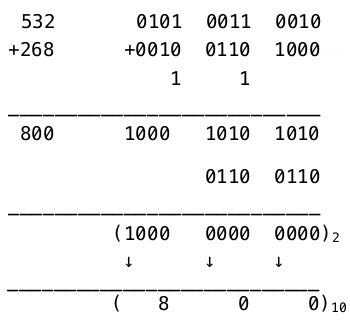
\includegraphics[scale=0.5]{ch2/image1}
\end{table}
\subsection{Codes non-pondérés}
\subsubsection{Code Gray}
Le code Gray est un code suivant le principe de \textit{Look-up Table}, c'est-à-dire que la conversion ne suit pas une règle mais une table de correspondance associant des valeurs. Le principe du Gray est que 2 codes voisins ne diffèrent que par la valeur d'un bit.
\begin{table}[H]
	\centering
	\begin{tabular}{c|c}
		Décimal & Gray \\
		\hline
		0 & 000\\
		 \hline
		1 & 001\\
		 \hline
		2 & 011\\
		 \hline
		3 & 010\\
		 \hline
		4 & 110\\
		 \hline
		5 & 111\\
		 \hline
		6 & 101\\
		 \hline
		7 & 101		 
	\end{tabular}
	\caption{Code Gray}
\end{table}
\subsubsection{Code ASCII}
Le code ASCII est utilisé pour coder les caractères dans des systèmes de traitement numérique, comme les majuscules, les signes de ponctuation et cetera. Le code est basé sur 8 bits, donc 256 possibilités, mais en réalité, on en utilise que 128.
\begin{figure}[H]
	\centering
	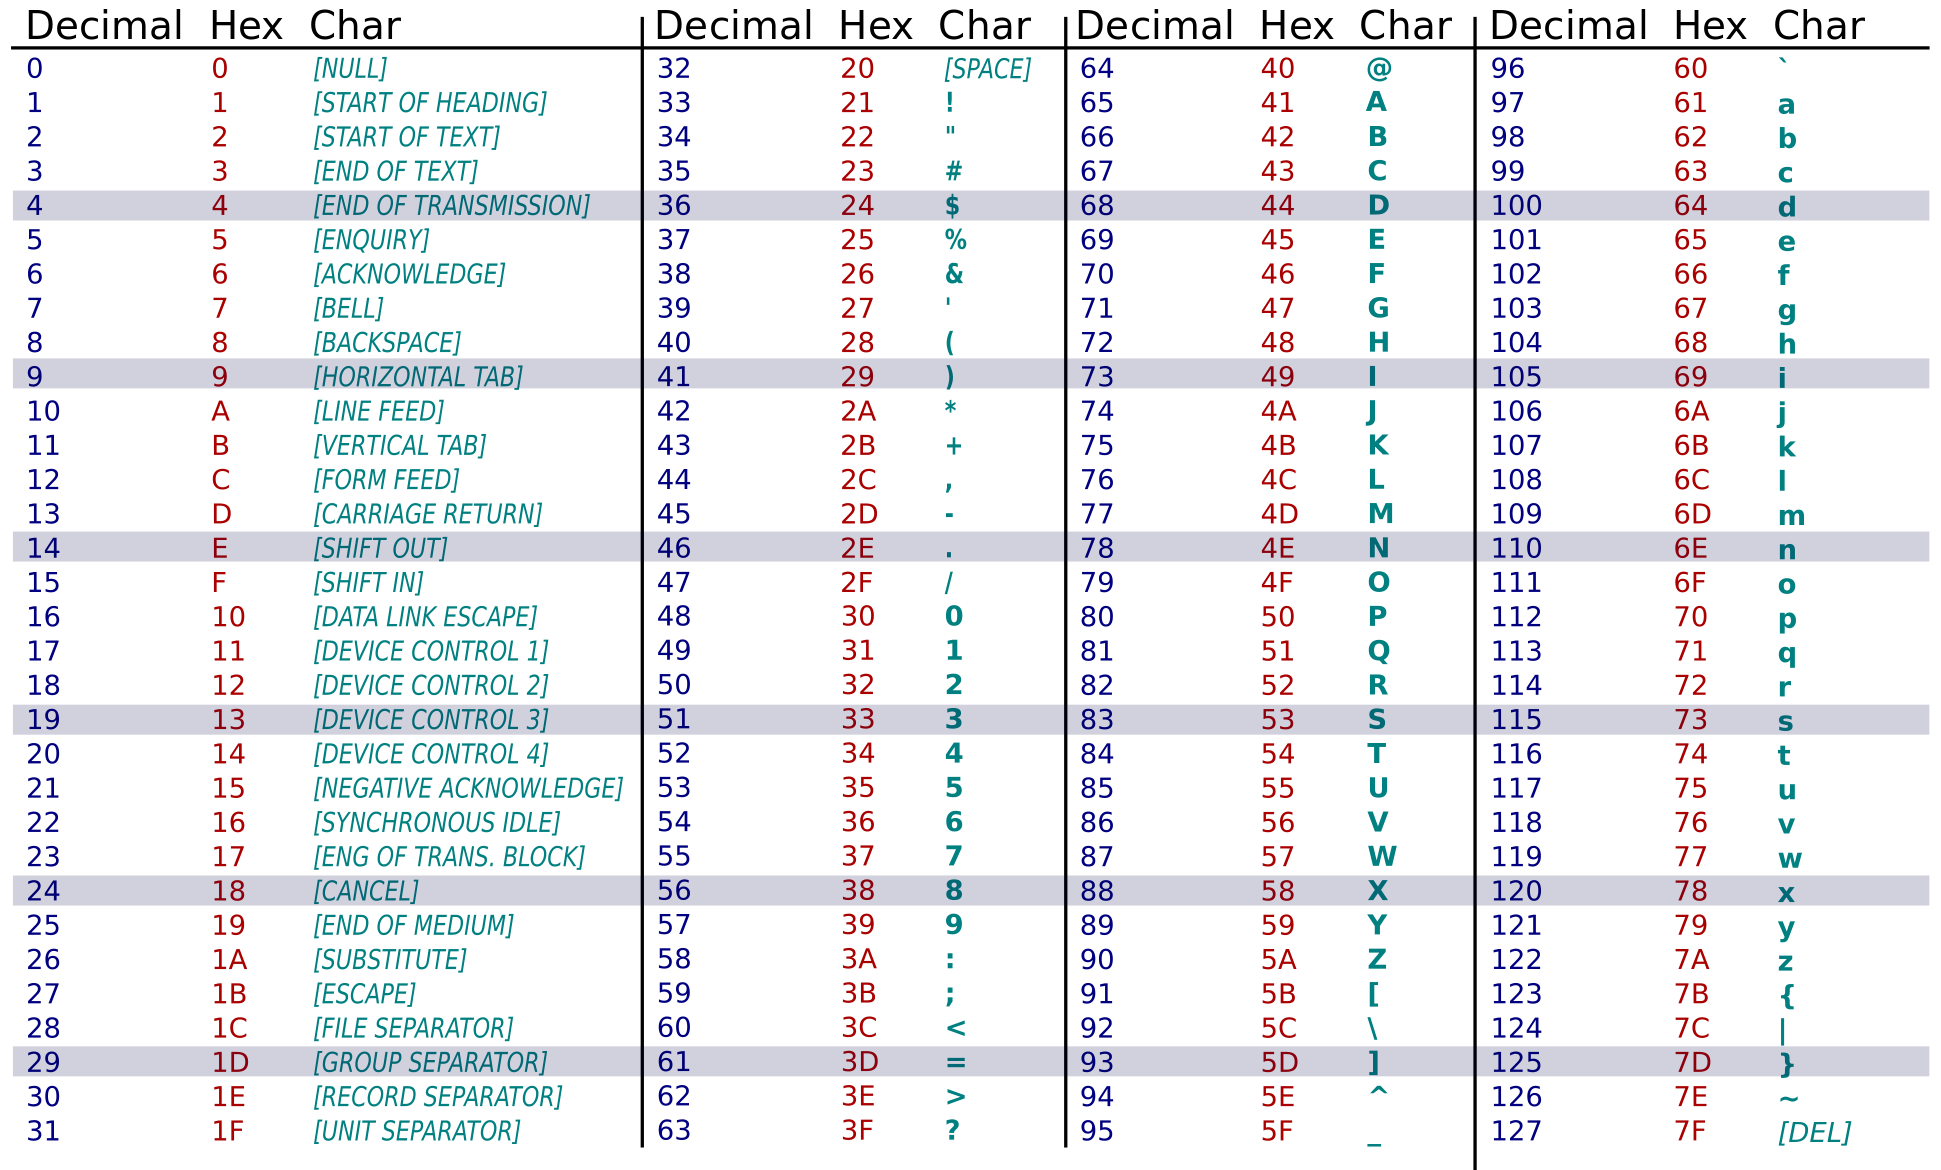
\includegraphics[width=\textwidth]{ch2/image2}
	\caption{Table ASCII}
\end{figure}
\subsection{Codes correcteurs}
\paragraph{Distance de Hamming} quantifie la distance (la différence)entre 2 séquences de symboles (ex : $d(0111,1010)=3$).
\paragraph{n-cube} cube à n dimensions ($2^n$ sommets) où chaque n-bit string est représenté par un des sommets. Les sommets adjacents ont une distance de Hamming de 1.
\begin{figure}[H]
	\centering
	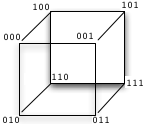
\includegraphics[scale=0.6]{ch2/image3}
	\caption{n-cube pour $n=3$}
\end{figure}
\subsubsection{Principe général}
Sur n-bits, on peut coder $2^n$ mots différents, si on rajoute 1 bit, nous avons $n$ mots supplémentaires. Nous pouvons donc grâce à cela, définir n mots qualifié d'erronés, ce qui sera utile pour détecter les erreurs (comme des erreurs de transmission).
\subsubsection{Codes de parité paire ou impaire (\textit{even (odd) parity codes})}
On code les mots de n-bits sur $(n+1)$ bits, ainsi nous avons autant de mots corrects que d'erronés. Le critère de correction est défini par le $(n+1)$\up{ème} bit.\\

Il faut compter le nombre de \textbf{1} et suivre la convention définie. Les 2 conventions sont: 
\begin{itemize}
	\item Bit de parité paire: 1 si c'est un nombre \textbf{impair}
	\item Bit de parité impair: 1 si c'est un nombre \textbf{pair}
\end{itemize}
Lors du calcul de parité, on peut ou non tenir compte du bit de parité (le $(n+1)$\up{ème}). Ici, on en tiendra pas compte.\\

Ce qui est intéressant, c'est de rajouter un bit de parité pour chaque poids (pour m-mits de n-bits, nous aurions donc des mots de $n+1$ pour le bit de parité et $m+1$ mot pour le bit de parité de poids). Ainsi, nous pourrions déterminer exactement le bit qui est erroné.
\begin{figure}[H]

	\begin{minipage}{0.55\textwidth}
	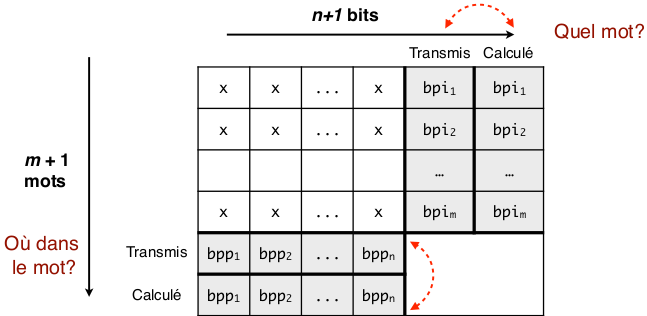
\includegraphics[scale=0.4]{ch2/image4}
	\end{minipage}
	\begin{minipage}{0.5\textwidth}
		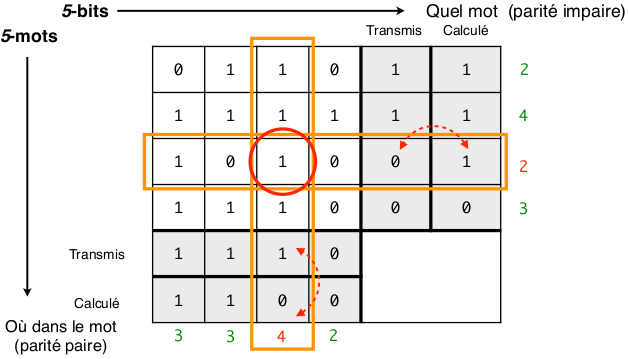
\includegraphics[scale=0.4]{ch2/image5}
	\end{minipage}
\end{figure}

\section{Algèbre de Boole}
\subsection{Définition}
Algèbre de Boole est un quadruplet $\{B,',\cdot,+\}$ où
$\left\{
\begin{array}{l l}
	B & \text{est un ensemble de 2 valeurs}\\
	' & \text{est l'opérateur de complément (parfois symbole \ $\bar{ }$ )}\\
	\cdot & \text{est l'opérateur \textbf{et}}\\
	+ & \text{est l'opérateur \textbf{ou}}
\end{array}\right.$\\\\
En fonction des définitions des opérateurs, on peut définir plusieurs algèbre de Boole. On ne s'intéressera ici que de celle-ci pour 2 valeurs.
\subsection{Algèbre de Boole à 2 valeurs}
\subsubsection{Définition}
L'algèbre de Boole à 2 valeurs est défini par (introduite par \textsc{Shannon}):
\begin{itemize}
	\item[$B=$]$\{0,1\}$
	\begin{itemize}
		\item[$0=$]faux
		\item[$1=$] vrai
	\end{itemize}
	\item[$+$]ou inclusif (or)
	\item[$\cdot$]et (and)
\end{itemize}
Les opérateurs $+$ et $\cdot$ peuvent être définis par \textbf{Tables de Vérités} (\textit{TdV}) suivantes:
\begin{table}[H]
	\begin{minipage}{0.5\textwidth}
		\centering
	$\begin{array}{c|c|c}
		x & y &  x\cdot y\\
		\hline
		0 & 0 & 0\\
		0 & 1 & 0\\
		1 & 0 & 0\\
		1 & 1 & 1
	\end{array}$
	\end{minipage}
	\begin{minipage}{0.5\textwidth}
		\centering
		$\begin{array}{c|c|c}
		x & y &  x+y\\
		\hline
		0 & 0 & 0\\
		0 & 1 & 1\\
		1 & 0 & 1\\
		1 & 1 & 1
		\end{array}$
	\end{minipage}
\end{table}
\subsubsection{Axiomes}
E. V. \textsc{Huntigton} posa 6 axiomes pour le cas de l'algèbre de Boole à 2 valeurs $B=\{0,1\}$. Ces axiomes sont vérifiables par \textit{TdV}. Les axiomes sont:
\begin{itemize}
	\item[Axiome 1] $B$ est \textbf{fermé} pour $+$ et pour $\cdot$
	\item[Axiome 2] $B$ a un \textbf{neutre} pour $+$ (noté $0$) et pour $\cdot$ (noté $1$)
	\item[Axiome 3] $B$ est \textbf{commutatif} par rapport à $+$ et $\cdot$
	\item[Axiome 4] $\cdot$ \textbf{distribue} $+$ et $+$ distribue $\cdot$
	\item[Axiome 5] $\exists$ \textbf{complément} de x (noté $x'$, $\bar{x}$ ou not($x$))
	\item[Axiome 6] Il y a au moins 2 éléments $x,y$ du $B$ tels que $x\neq y$
\end{itemize}
L'une des conséquence de ces axiomes est l'\textbf{associativité}
\begin{equation}
	(a+b)+c=a+(b+c)\quad\text{et}\quad(a\cdot b)\cdot c=a\cdot(b\cdot c)
\end{equation}
\subsubsection{Théorèmes}
À partir de ces axiomes, nous pouvons définir les théorèmes suivants:
\begin{itemize}
	\item[Théorème 1]
	\item[Théorème 2]
	\item[Théorème 3]
	\item[Théorème 4]
	\item[Théorème 5]
	\item[Théorème 6]
	\item[Théorème 7]
\end{itemize}
\section{Fonctions logiques}

\section{Réalisation matérielle}
